%!TEX root = ../these.tex

\chapter{
  Описание формата файлов DBS
}
\label{app:dbs}

\newcommand{\dbsRecord}[1]{
  \noindent
  \begin{tabularx}{\textwidth}{|>{\raggedleft}p{3em}|>{\centering}p{4em}|p{3em}|X|}
    \hline
    \multicolumn{1}{|c|}{Смещение} &
    \multicolumn{1}{c|}{Тип}      &
    \multicolumn{1}{c|}{Имя}      &
    \multicolumn{1}{c|}{Описание}     \\
    \hline
    #1
    \\
    \hline
  \end{tabularx}
}

\dbsRecord{
  +4 & text & 5 & Превед Медвед! \\
  +12 & i16 & 7 & Пока!
}

\begin{figure}
  \centering
  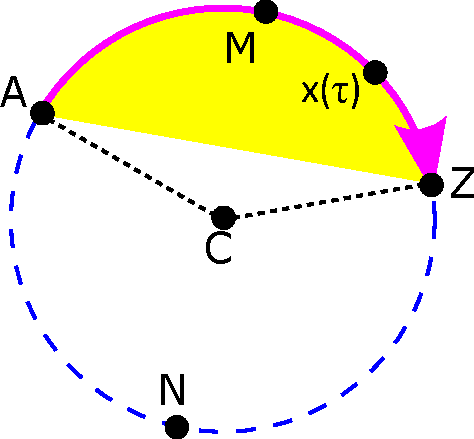
\includegraphics{arc.pdf}
  \caption{Дуга}
  \label{fig:app.arc}
\end{figure}
